\documentclass[10pt]{ctexart}
\usepackage[a4paper,margin=0.85in]{geometry}
\usepackage{amsmath,amssymb,booktabs,array}
\usepackage{enumitem}
\usepackage{listings}
\usepackage{xcolor}
\usepackage{microtype}
\usepackage{graphicx}
\usepackage{hyperref}
\graphicspath{{../figures/}{EXPS/figures/}}
\setlist[itemize]{leftmargin=1.5em}
\setlist[enumerate]{leftmargin=1.8em}
\lstset{basicstyle=\ttfamily\scriptsize,breaklines=true,columns=fullflexible,keepspaces=true,frame=single,framerule=0.2pt,xleftmargin=0.5em,xrightmargin=0.5em}
\title{018：StepPPO-v3 Value-Head-Only 完整实验分析}
\author{}
\date{2026-06-10}
\begin{document}
\maketitle
\vspace{-1.2em}

\section*{摘要结论}
这次 StepPPO-v3 完整跑到 \textbf{global step 250}。从 value diagnostics 看，value head 的学习信号非常明确：pred-target correlation、normalized RMSE、prediction scale matching、full-batch explained variance 和 sample-level ranking 都持续改善。因此，\textbf{v3 的核心问题“actor-side shared value head 能不能学到 step-level return/value signal”目前答案是 yes。}

但是，这次完整 run 使用的是 \path{detach_value_backbone=False}。它允许 value loss 回传 actor backbone。结果表明 policy 没有崩，但后期 actor 行为出现明显漂移：response length 和 response clip ratio 大幅升高，导致 generation time 和 total step time 变慢，并且 task score 相比 GiGPO baseline 有下降。因此，\textbf{这次 run 支持“value head 可学习”，但不支持“detach=false 完全不影响 GiGPO”。}

\section{StepPPO-v3 的实现原理}
本节先把 v3 的代码设计讲清楚，使后面的指标分析可以自包含地理解。

\subsection{v3 的定位：value-head-only，不改 GiGPO policy}
当前分支中的 StepPPO-v3 不是一个新的 policy-gradient estimator，也不是把 step-level value 直接接入 policy advantage 的算法。它的实验目标很窄：
\begin{itemize}
  \item 保持 GiGPO 原本的 rollout、policy advantage、policy loss 和 PPO ratio 路径不变。
  \item 在 actor 侧额外加一个 shared value head，用来预测 step-level value/return target。
  \item 检查两个问题：第一，value head 能不能稳定学到 step-level target；第二，加入这个 auxiliary loss 后，会不会损害 GiGPO 原本训练行为。
\end{itemize}

因此，训练时 actor 的 policy loss 仍然由 GiGPO 的 advantage 决定。value head 的损失只是一个 auxiliary loss：它不会在这次 v3 中替代 GiGPO advantage，也不会直接改变 action-level PPO ratio。

\subsection{value 是怎么得到的}
每一个 WebShop episode 可以看成一个多步交互轨迹。第 $i$ 个 step 在生成 action 之前有一段 context，包括任务、历史 observation、历史 action 和当前 observation。模型对这段 context 做 forward 后，会得到每个 token 的 hidden state。v3 只选取一个 hidden state 作为 step-level 表示：
\begin{equation}
  h_i = h_{\text{pre-action-last-context-token}}.
\end{equation}

直观上，$h_i$ 是模型在“准备生成当前 step action 之前”对当前状态的表示。value head 只接收这个 selected hidden state，而不是所有 token 的 hidden states：
\begin{equation}
  v_i = f_\phi(h_i),
\end{equation}
其中 $f_\phi$ 是一个很小的 MLP value head，输出 scalar prediction $v_i \in \mathbb{R}$。这个 scalar 被解释为当前 step 的 predicted step-level return/value。

\subsection{value target 是什么}
v3 使用 step-level return target，而不是 final episode reward 的直接 copy。记 step-level reward 为 $r_i$，bootstrapped/GAE-style target 记为 $y_i$。代码中该 target 对应 diagnostics 里的 \path{value_target_gae_return}。可以把它理解成当前 step 往后能获得多少 normalized/discounted return 的训练标签。

简化地说，target 的构造类似：
\begin{equation}
  y_i \approx \sum_{k \ge i} \gamma^{k-i} \lambda^{k-i} r_k,
\end{equation}
本次实验配置中使用 \path{step_gamma=0.95} 和 \path{step_lam=0.90}。实际实现还会结合 trajectory 内 step reward、valid action penalty 和 batch 组织方式，但核心含义就是：用未来 step-level return 监督 value head。

\subsection{value loss 如何加入 actor update}
value head 的基本优化目标是让 prediction $v_i$ 接近 target $y_i$。不考虑 clipping 时，最简单形式是 MSE：
\begin{equation}
  \mathcal{L}_{\mathrm{value}} = \frac{1}{N}\sum_{i=1}^{N} (v_i - y_i)^2.
\end{equation}
代码里还保留了 PPO-style value clipping，对应配置 \path{cliprange_value=0.5}，用于限制单次 value update 的过大变化。总 actor-side loss 可以抽象成：
\begin{equation}
  \mathcal{L}_{\mathrm{actor}} = \mathcal{L}_{\mathrm{GiGPO\ policy}} + c_v \mathcal{L}_{\mathrm{value}} + \text{KL/entropy/penalty terms},
\end{equation}
本次 $c_v=0.03$。

\subsection{detach\_value\_backbone 的含义}
\path{detach_value_backbone} 决定 value loss 是否回传到 actor backbone：
\begin{itemize}
  \item 若 \path{detach_value_backbone=True}，value head 看到的是 detached hidden state。value loss 只更新 value head 参数，不更新 actor backbone。这个设置更适合验证“value head 自身能否从固定 actor representation 中读出 value signal”，也更安全，因为它较少干扰 GiGPO policy。
  \item 若 \path{detach_value_backbone=False}，value loss 会回传到产生 $h_i$ 的 actor backbone。这个设置可能让 representation 更适合 value prediction，但也可能改变 policy 的 hidden representation，从而影响 GiGPO 的行为分布。
\end{itemize}

本次完整实验使用 \path{detach_value_backbone=False}。因此，本报告后面对 actor drift 的分析非常重要：如果后期 policy 行为变差或生成变长，不能排除 auxiliary value loss 对 backbone 的影响。

\section{实验数据和对照设置}
本次分析把 v3 的完整训练轨迹定义为：初始 run 的 step 1--100 加上 resume run 的 step 101--250。第一次 run 在 121/122 左右中断，但最后保存的 checkpoint 是 step 100；resume 从 step 100 checkpoint 继续，因此 step 101--121 应以 resume run 为准。

\begin{lstlisting}
# v3 stage-1 log, use steps 1--100
logs/webshop_gigpo_v1_value_aux_step_ppo_v3_value_head_detach_false_qwen25_15b_4gpu_paper_align_simple_20260609_070507.log

# v3 resume log, use steps 101--250
logs/webshop_gigpo_v1_value_aux_step_ppo_v3_value_head_detach_false_qwen25_15b_4gpu_paper_align_simple_20260610_012702.log

# v3 diagnostics, use stage-1 1--100 and resume 101--250
logs/value_diagnostics/step_ppo_v3_value_head_detach_false_qwen2.5_1.5b_4gpu_paper_align_full_e250/
logs/value_diagnostics/step_ppo_v3_value_head_detach_false_qwen2.5_1.5b_4gpu_paper_align_full_e250_resume_20260610_012700/
\end{lstlisting}

GiGPO 对照采用已有三 seed 完整 baseline：
\begin{lstlisting}
logs/webshop_gigpo_qwen25_15b_4gpu_paper_align_simple_20260530_114442.log
logs/webshop_gigpo_qwen25_15b_4gpu_paper_align_simple_20260531_004613.log
logs/webshop_gigpo_qwen25_15b_4gpu_paper_align_simple_20260531_123134.log
\end{lstlisting}

所有窗口统计均按 50 step 分段：1--50、51--100、101--150、151--200、201--250。value diagnostics 使用每 step 的 full-batch summary；sample-level ranking 使用每 step dump 的最多 512 条 sample rows。

\section{Value learning 指标定义}
为了判断 value head 是否“学到了”，不能只看 raw value loss。原因是 target $y_i$ 本身是 non-stationary 的：policy 变好后 reward/return 的尺度会变大，MSE 可能因为 target scale 变大而上升。下面定义的指标更能区分“模型是否真正捕捉了 target 结构”。

\subsection{Pred-target correlation}
给定一个 batch 中的 prediction $v_i$ 和 target $y_i$，Pearson correlation 定义为：
\begin{equation}
  \rho(v,y) = \frac{\sum_i (v_i - \bar v)(y_i - \bar y)}{\sqrt{\sum_i (v_i - \bar v)^2}\sqrt{\sum_i (y_i - \bar y)^2}}.
\end{equation}

它衡量 prediction 和 target 的线性相关程度。若 value head 只是输出常数，prediction variance 很小，correlation 会接近 0 或不稳定。若 value head 学会“哪些状态的未来 return 更高，哪些更低”，correlation 应该上升。

Correlation 对 value learning 很重要，因为 value function 的第一步能力就是\textbf{排序/区分状态好坏}。即使 absolute calibration 暂时不准，只要 correlation 持续提升，就说明 representation 和 value head 已经捕捉到 return-related signal。

\subsection{RMSE 和 NRMSE}
RMSE 定义为：
\begin{equation}
  \mathrm{RMSE} = \sqrt{\frac{1}{N}\sum_{i=1}^{N}(v_i-y_i)^2}.
\end{equation}

但是 raw RMSE 会受 target 尺度影响。若 $y_i$ 的 standard deviation 从 1 增到 4，即使模型相对误差变小，raw RMSE 也可能变大。因此我们使用 normalized RMSE：
\begin{equation}
  \mathrm{NRMSE} = \frac{\mathrm{RMSE}}{\mathrm{Std}(y)}.
\end{equation}

NRMSE 的直觉是：prediction error 相对于 target 自身波动有多大。若 NRMSE 约等于 1，说明误差和 target 的自然波动同量级；若明显小于 1，说明 prediction 已经解释了 target 中相当一部分结构。NRMSE 下降比 raw loss 下降更能说明 value head 在 non-stationary RL 训练中学到了东西。

\subsection{Prediction std / target std}
这个指标定义为：
\begin{equation}
  \mathrm{StdRatio} = \frac{\mathrm{Std}(v)}{\mathrm{Std}(y)}.
\end{equation}

它衡量 prediction 的动态范围是否接近 target。如果 value head 输出近似常数，则 $\mathrm{Std}(v)$ 很小，StdRatio 接近 0。若 value head 开始覆盖 target 的高低变化，StdRatio 会接近 1。当然，StdRatio 接近 1 本身不保证正确，因为 prediction 可能有方差但方向错；所以它必须和 correlation 一起看。理想情况是：correlation 高，同时 StdRatio 接近 1。

\subsection{Full-batch explained variance}
这里使用 diagnostics 的 full-batch RMSE 和 target std 计算 implied explained variance：
\begin{equation}
  \mathrm{EV} = 1 - \frac{\mathrm{MSE}}{\mathrm{Var}(y)} = 1 - \mathrm{NRMSE}^2.
\end{equation}

EV 的意义是 prediction 解释了 target variance 的多少。EV=0 表示和只预测 target mean 差不多；EV$>0$ 表示优于常数 baseline；EV 越接近 1 越好。actor console log 里的 \path{actor/value_explained_variance} 是 microbatch 上算的，容易受小 batch 和 target variance 波动影响，所以本报告更信任 diagnostics 的 full-batch EV。

\subsection{Normalized bias}
Bias 定义为 prediction error 的均值：
\begin{equation}
  \mathrm{Bias} = \frac{1}{N}\sum_i (v_i-y_i), \qquad
  \mathrm{NormBias}=\frac{\mathrm{Bias}}{\mathrm{Std}(y)}.
\end{equation}

它衡量 value head 是否整体高估或低估。Correlation 高但 bias 很大，说明排序可能学到了，但 calibration 仍不准。因此 bias 是 calibration 的补充指标。

\section{Value head 是否学到了？}
结论是明确的：\textbf{学到了，而且越到后期越明显。}

\begin{center}
\begin{tabular}{lrrrrr}
\toprule
Metric / Window & 1--50 & 51--100 & 101--150 & 151--200 & 201--250 \\
\midrule
Pred-target corr & 0.144 & 0.493 & 0.766 & 0.811 & 0.861 \\
NRMSE & 1.021 & 0.885 & 0.654 & 0.588 & 0.508 \\
Pred std / target std & 0.064 & 0.441 & 0.822 & 0.855 & 0.936 \\
Full-batch EV & -0.043 & 0.205 & 0.559 & 0.644 & 0.723 \\
\bottomrule
\end{tabular}
\end{center}

这四行指标共同构成比较强的证据链：
\begin{itemize}
  \item \textbf{Correlation 上升}说明 prediction 与 target 的方向越来越一致，value head 开始能区分高 return 和低 return step。
  \item \textbf{NRMSE 下降}说明误差相对 target 自身波动越来越小，不是仅仅因为 target scale 改变导致的假象。
  \item \textbf{StdRatio 接近 1}说明 value head 不再输出被压缩的近似常数，而是开始覆盖 target 的动态范围。
  \item \textbf{Full-batch EV 从负到正并持续上升}说明 prediction 从不如常数 baseline，变成能解释 target variance 的 predictor。
\end{itemize}

因此，虽然 raw \path{actor/value_loss} 不是单调下降，仍然可以判断 value head 在学习。特别是 201--250 窗口，corr=0.861、NRMSE=0.508、StdRatio=0.936、EV=0.723，这已经是比较明显的可学习信号。

Selected steps 也能看到同样趋势：
\begin{center}
\begin{tabular}{rrrrrr}
\toprule
Step & Corr & NRMSE & Full EV & Std Ratio & Bias / Std \\
\midrule
1 & -0.042 & 1.120 & -0.254 & 0.140 & -0.472 \\
50 & 0.461 & 0.975 & 0.049 & 0.094 & -0.167 \\
100 & 0.674 & 0.749 & 0.439 & 0.686 & 0.123 \\
150 & 0.717 & 0.728 & 0.470 & 0.804 & -0.192 \\
200 & 0.933 & 0.369 & 0.864 & 0.888 & 0.073 \\
225 & 0.955 & 0.302 & 0.909 & 0.950 & -0.051 \\
250 & 0.872 & 0.515 & 0.735 & 0.916 & 0.150 \\
\bottomrule
\end{tabular}
\end{center}

Step 250 比 step 225 稍有回落，但仍明显优于早期。这种单步波动在 RL 训练中正常，因为每个 batch 的 tasks、episode outcomes 和 target distribution 都不同。更可靠的是窗口均值趋势。

\section{Sample-level ranking 的定义和意义}
Batch-level correlation 可能掩盖一些问题：例如 prediction 在 batch 内整体相关，但在具体 sample 层面并不能稳定地区分好坏。为了进一步验证，我们使用 dumped rows 做 sample-level ranking analysis。

具体做法如下：
\begin{enumerate}
  \item 收集一个窗口内所有 dumped samples，每个 sample 有 prediction $v_i$ 和 target $y_i$。
  \item 按 prediction $v_i$ 从低到高排序。
  \item 将 samples 分成五个等量 quintiles：Q1 是 prediction 最低的 20\%，Q5 是 prediction 最高的 20\%。
  \item 计算每个 quintile 的平均 target return。
  \item 如果 value head 有用，那么 Q5 的平均 target 应该显著高于 Q1，并且 target 应随 quintile 大致单调上升。
\end{enumerate}

这个指标检验的是 value head 是否能在 sample 层面对状态做排序。它比只看 MSE 更贴近 value function 在 RL 中的用途：value 需要告诉我们哪些状态/step 更有希望，哪些更差。

\begin{center}
\begin{tabular}{lrrrr}
\toprule
Window & Pearson & Spearman & NRMSE & Top-bottom target gap \\
\midrule
1--50 & 0.381 & 0.760 & 0.936 & 2.454 \\
51--100 & 0.520 & 0.553 & 0.857 & 5.415 \\
101--150 & 0.780 & 0.823 & 0.630 & 8.433 \\
151--200 & 0.814 & 0.858 & 0.584 & 8.734 \\
201--250 & 0.873 & 0.909 & 0.492 & 9.112 \\
\bottomrule
\end{tabular}
\end{center}

这里 Pearson correlation 衡量线性相关；Spearman correlation 衡量 rank correlation，即 prediction 排名和 target 排名是否一致。Spearman 后期达到 0.909，说明排序能力非常强。Top-bottom target gap 从 2.454 增到 9.112，说明高 prediction quintile 对应的真实 target return 明显更高。

因此 sample-level ranking 的结论是：value head 不只是 batch summary 上“看起来相关”，它在 individual sample 层面也能把高 return step 和低 return step 分开。

\section{为什么 raw value loss 会误导}
在 supervised learning 中，loss 下降通常直接表示学得更好。但 RL 里的 value target 是 non-stationary 的：policy 变强后，episode reward、trajectory length、valid action ratio 和 return distribution 都会变化。若 target variance 变大，MSE/MAE 即使在相对意义上改善，也可能在绝对数值上不降反升。

因此，本实验里 raw \path{actor/value_loss} 的解释应当非常谨慎：
\begin{itemize}
  \item 若 target std 上升，raw RMSE 上升不一定代表 value 学坏了。
  \item 若 prediction std 也跟随 target std 上升，并且 correlation 上升，说明模型正在学习 target 的结构。
  \item 若 NRMSE 下降、EV 上升，则说明相对 target distribution 的误差确实在下降。
\end{itemize}

这也是为什么本报告把 corr、NRMSE、StdRatio、EV 和 sample-level ranking 作为主要判断依据，而不是只看 console log 中的 raw value loss。

\section{Actor 行为是否被影响}
value head 的另一个关键问题是：它是否影响了 GiGPO 原本训练。这里要区分“policy 是否崩掉”和“policy 是否完全不受影响”。本次结果是：\textbf{没有崩，但后期有明显 drift。}

\begin{center}
\begin{tabular}{lrrrr}
\toprule
Window & Metric & v3 & GiGPO mean & Delta \\
\midrule
1--50 & success & 0.156 & 0.155 & +0.001 \\
51--100 & success & 0.477 & 0.441 & +0.036 \\
101--150 & success & 0.647 & 0.623 & +0.024 \\
151--200 & success & 0.706 & 0.699 & +0.007 \\
201--250 & success & 0.717 & 0.736 & -0.019 \\
\midrule
1--50 & task score & 0.476 & 0.456 & +0.020 \\
51--100 & task score & 0.741 & 0.720 & +0.021 \\
101--150 & task score & 0.789 & 0.812 & -0.022 \\
151--200 & task score & 0.838 & 0.855 & -0.017 \\
201--250 & task score & 0.822 & 0.871 & -0.049 \\
\midrule
201--250 & valid action ratio & 0.947 & 0.997 & -0.050 \\
201--250 & response clip ratio & 0.426 & 0.0015 & +0.425 \\
201--250 & response length mean & 293.167 & 127.803 & +165.364 \\
\bottomrule
\end{tabular}
\end{center}

这些 actor 指标的含义如下：
\begin{itemize}
  \item \textbf{success rate}：episode 是否成功完成任务。它是最直观的最终指标，但比较粗糙。
  \item \textbf{task score}：WebShop 的连续评分，比 success 更细，可以反映部分匹配质量。
  \item \textbf{valid action ratio}：模型输出是否能被环境解析成合法 action。下降说明 action formatting 或策略稳定性变差。
  \item \textbf{response length / clip ratio}：模型输出长度和是否触达 max response length。clip ratio 高说明模型经常生成到长度上限，这通常是 actor 行为漂移或冗长推理的信号。
\end{itemize}

关键现象是 response length。前 150 step 基本可控，但 151 之后 clip ratio 开始升高，201--250 达到非常高的 0.426。这个变化比 success/task score 更值得重视，因为它说明 actor 的输出分布发生了明显变化。虽然 final success 没有大幅下降，但 task score、valid action ratio 和 runtime 都受到影响。

Validation 结果也支持这个更谨慎的判断：
\begin{center}
\begin{tabular}{lrrr}
\toprule
Validation metric & v3 @250 & GiGPO mean @250 & Delta \\
\midrule
Success rate & 0.742 & 0.752 & -0.010 \\
Task score & 0.843 & 0.885 & -0.042 \\
\bottomrule
\end{tabular}
\end{center}

如果只看最后 6 个 validation checkpoint（225--250），v3 success 平均 0.750，GiGPO 平均 0.743，success 不差；但 v3 task score 平均 0.837，GiGPO 平均 0.875，仍低约 0.037。因此不能只看 success，要同时看 task score、valid action ratio 和 response clipping。

\section{训练时间和资源分析}
value head 本身的 diagnostics dump 很轻，但这次总 runtime 后期明显变慢。主要原因不是每步 dump 文件，而是 actor 输出变长后 generation token 数增加。

\begin{center}
\begin{tabular}{lrrrr}
\toprule
Window & Metric & v3 & GiGPO mean & Ratio \\
\midrule
1--50 & step time & 164.0s & 163.9s & 1.00 \\
51--100 & step time & 133.3s & 148.3s & 0.90 \\
101--150 & step time & 150.1s & 117.8s & 1.27 \\
151--200 & step time & 173.2s & 104.2s & 1.66 \\
201--250 & step time & 189.9s & 105.1s & 1.81 \\
\midrule
201--250 & generation time & 165.3s & 88.0s & 1.88 \\
201--250 & actor update time & 16.1s & 11.3s & 1.43 \\
201--250 & throughput & 1742.1 & 2281.6 & 0.76 \\
\bottomrule
\end{tabular}
\end{center}

因此，“value head 会不会显著增加训练时间”需要拆开看：
\begin{itemize}
  \item diagnostics dump 开销很小，每步大约几十毫秒量级。
  \item actor update 末段从 GiGPO 的 11.3s 增到 16.1s，说明 value head/backbone update 确实带来一些训练开销。
  \item 最大 runtime 问题来自 generation 变长：201--250 的 generation time 是 baseline 的 1.88 倍，这和 response clip ratio 大幅升高一致。
\end{itemize}

\section{曲线总览}
\begin{figure}[h]
  \centering
  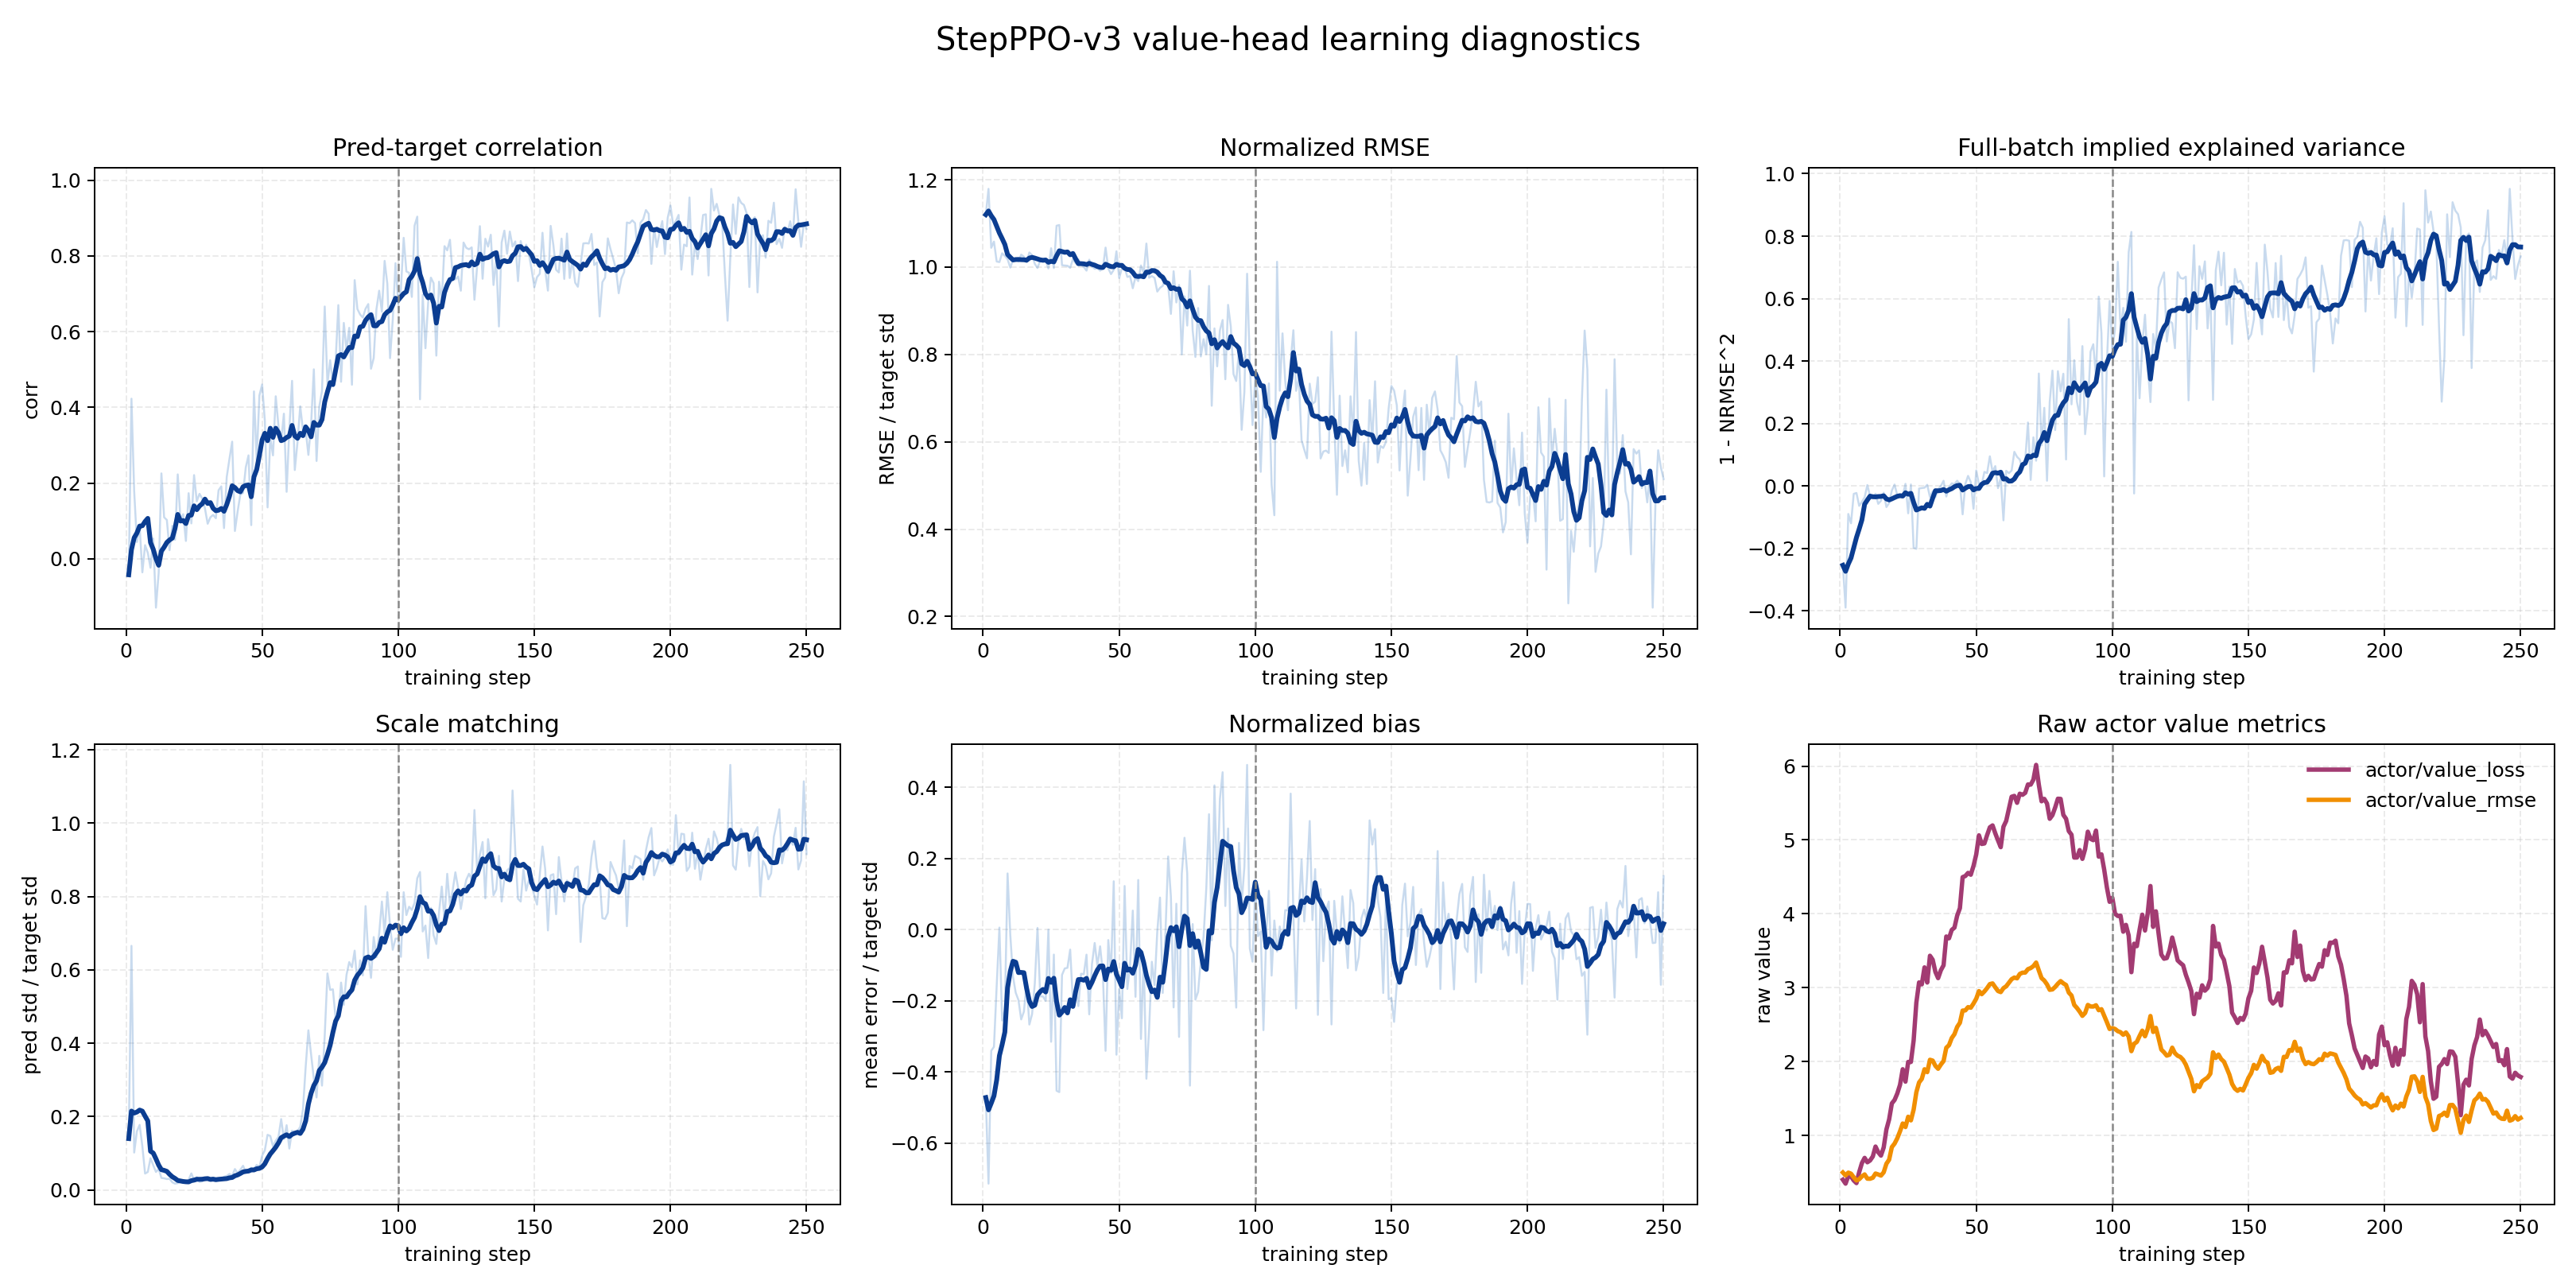
\includegraphics[width=\linewidth]{018_step_ppo_v3_value_learning_curves.png}
  \caption{Value head 学习曲线。灰色虚线为 step 100 resume 边界。}
\end{figure}

\begin{figure}[h]
  \centering
  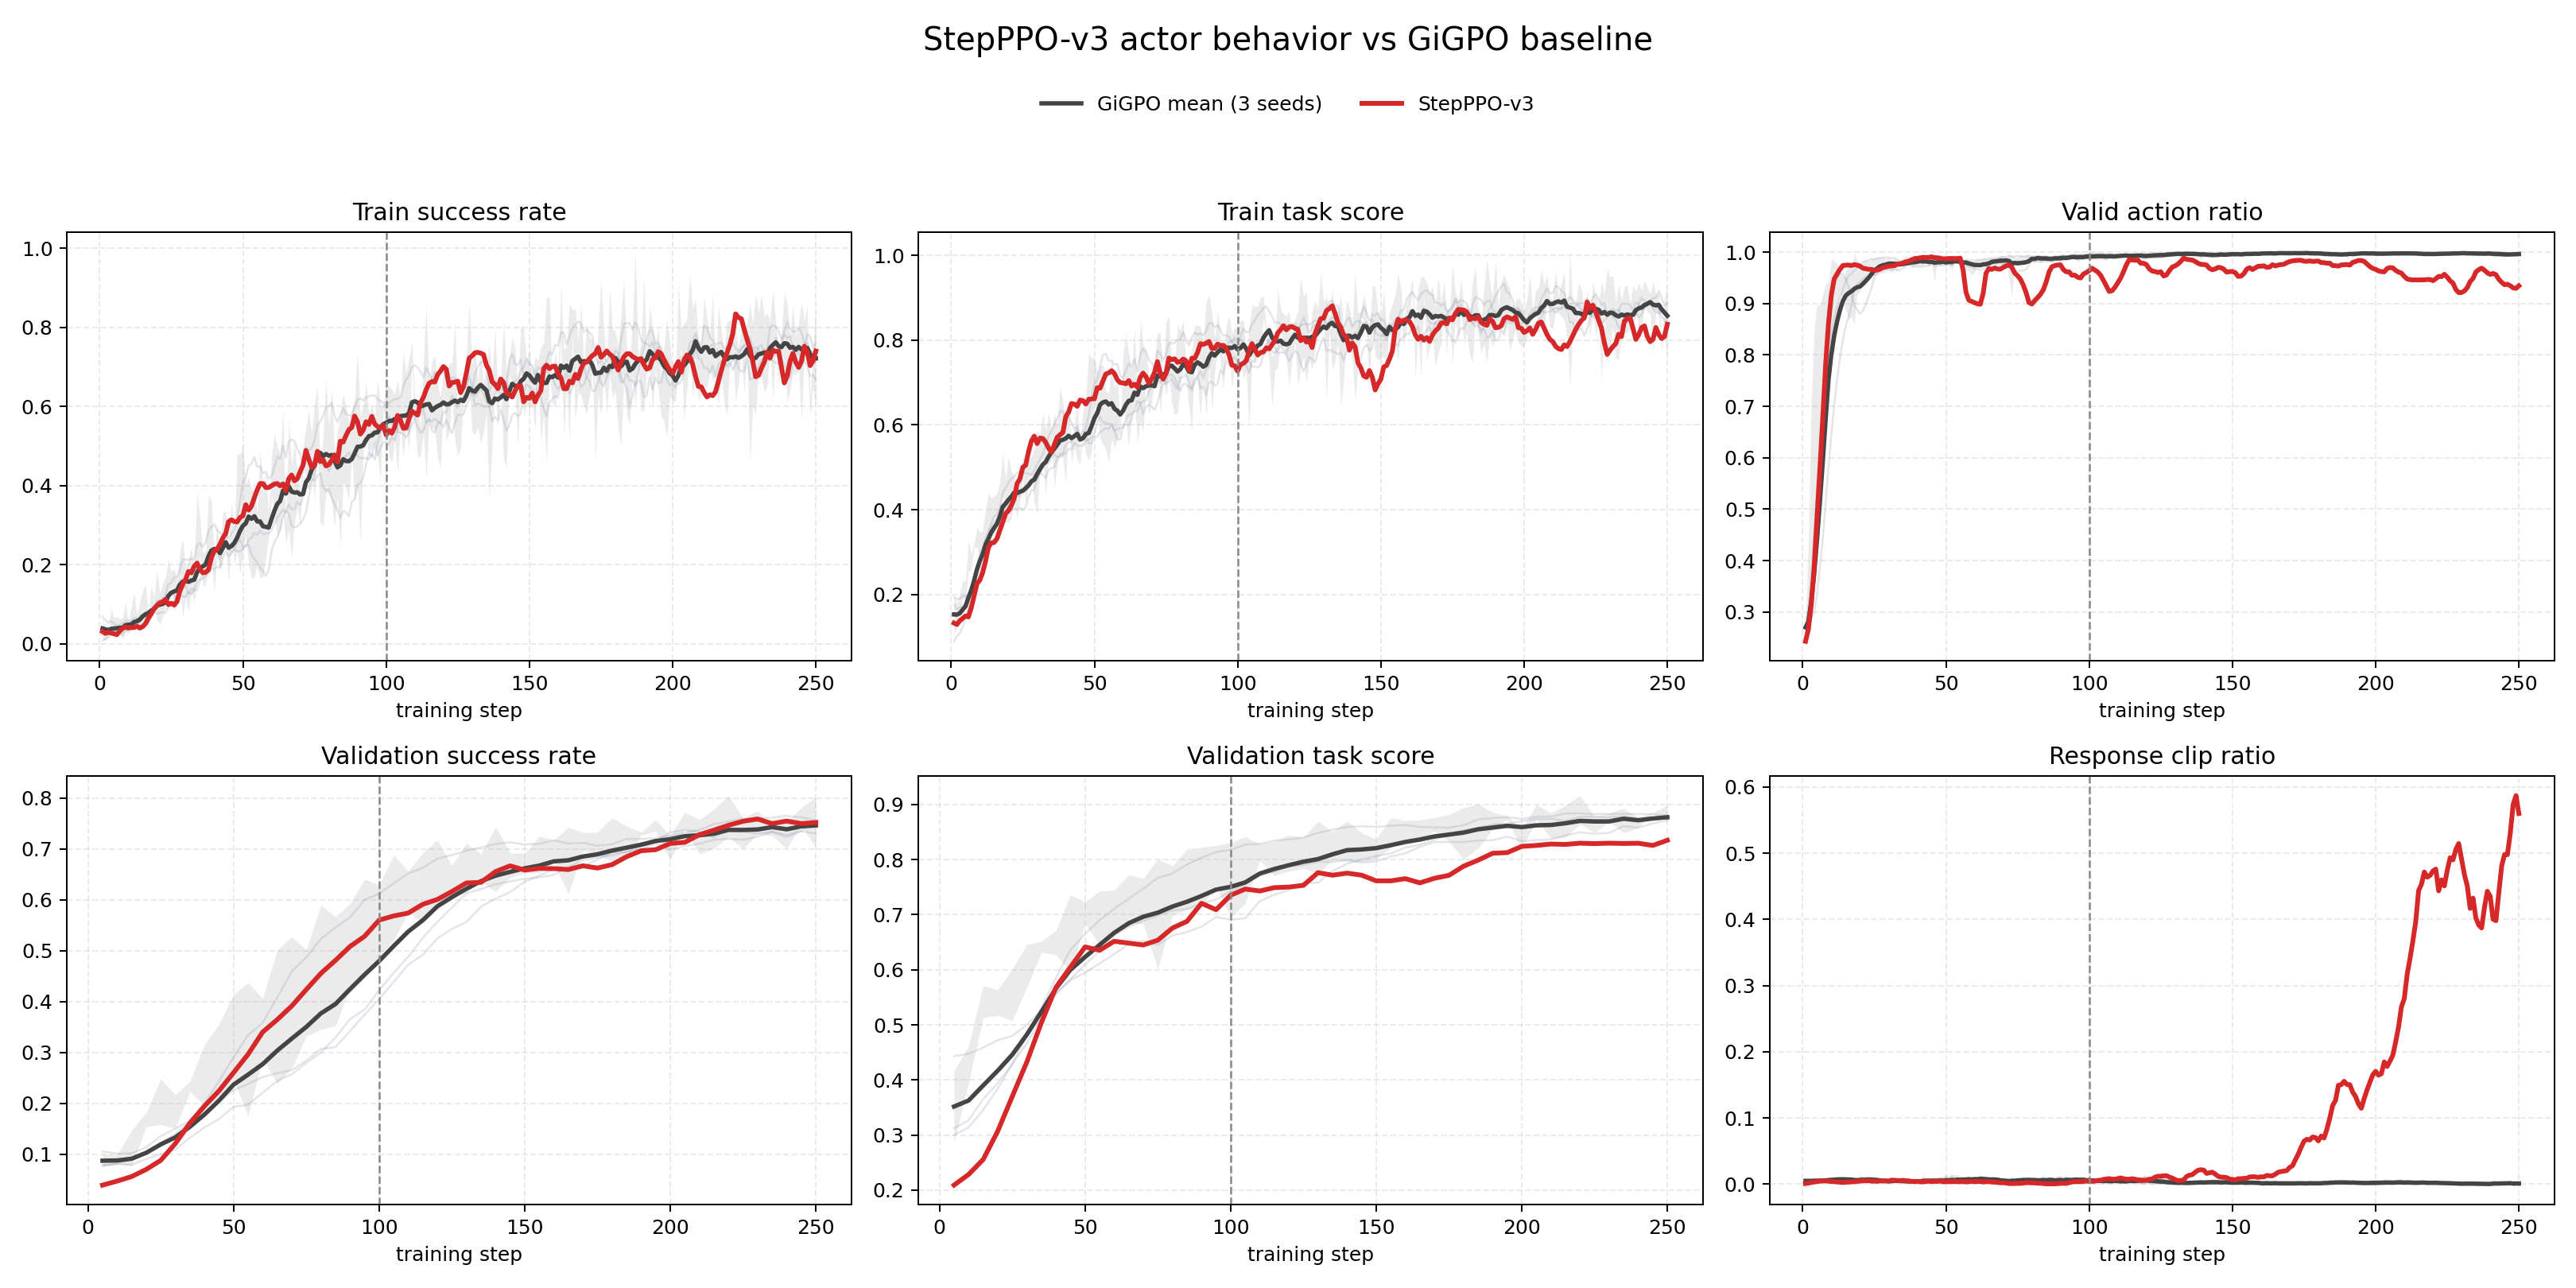
\includegraphics[width=\linewidth]{018_step_ppo_v3_policy_vs_gigpo_curves.png}
  \caption{v3 actor 行为与 GiGPO 三 seed baseline 对比。}
\end{figure}

\begin{figure}[h]
  \centering
  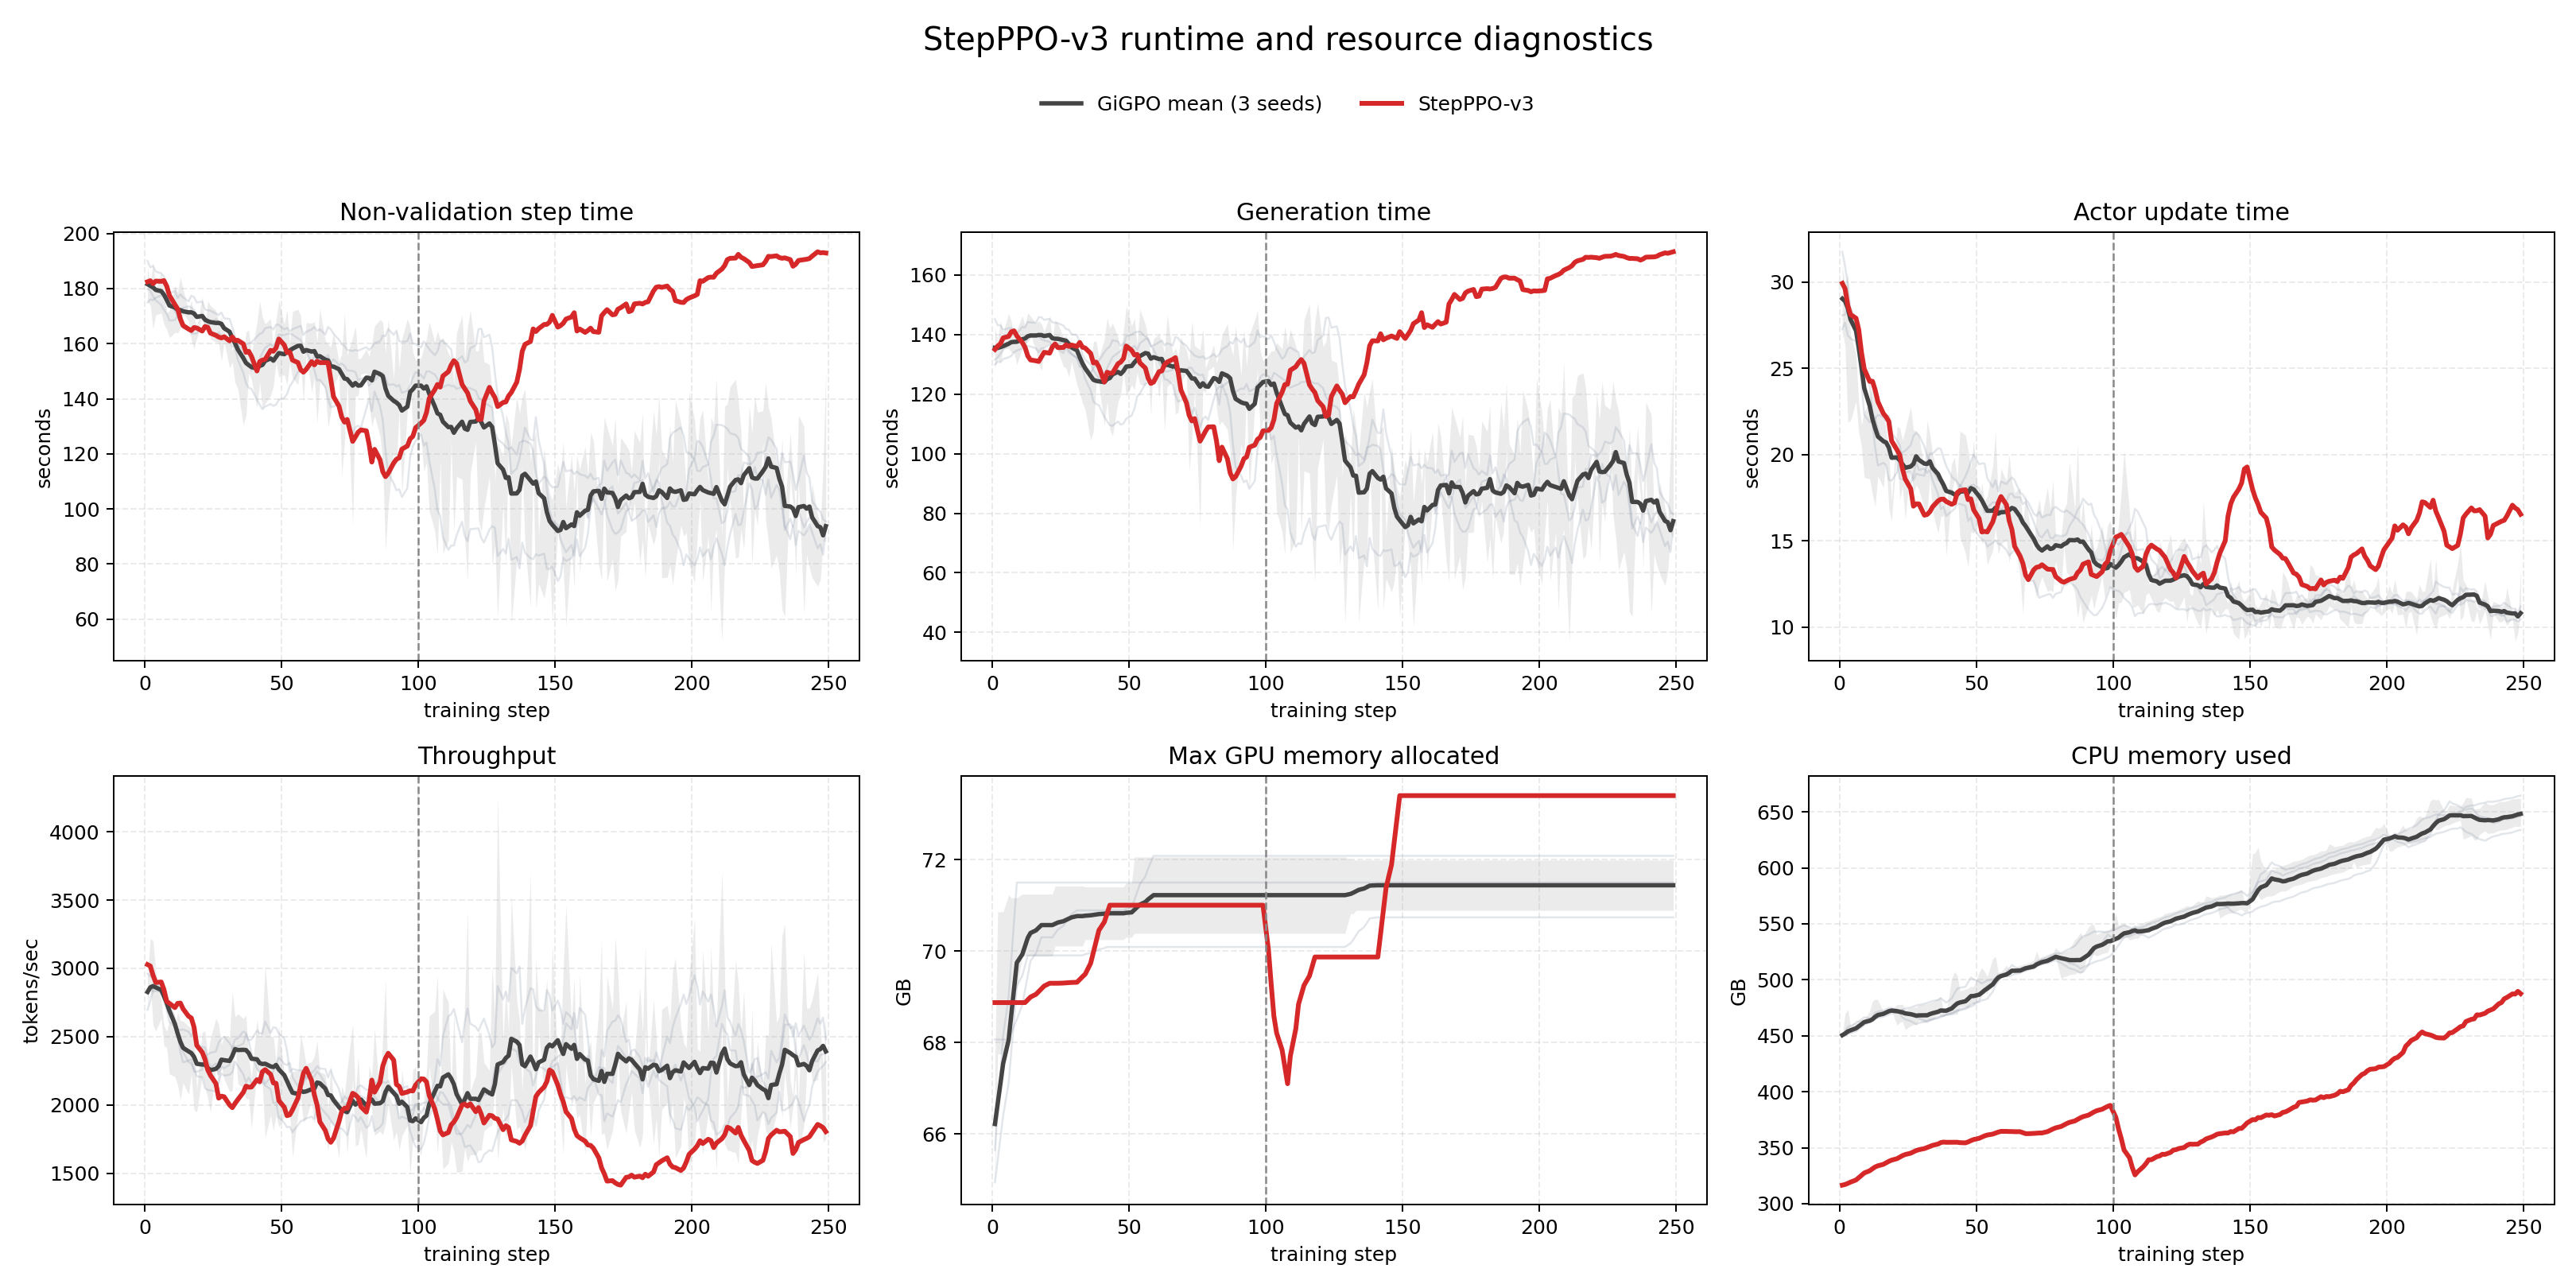
\includegraphics[width=\linewidth]{018_step_ppo_v3_runtime_resource_curves.png}
  \caption{v3 runtime/resource 与 GiGPO 三 seed baseline 对比。}
\end{figure}

\begin{figure}[h]
  \centering
  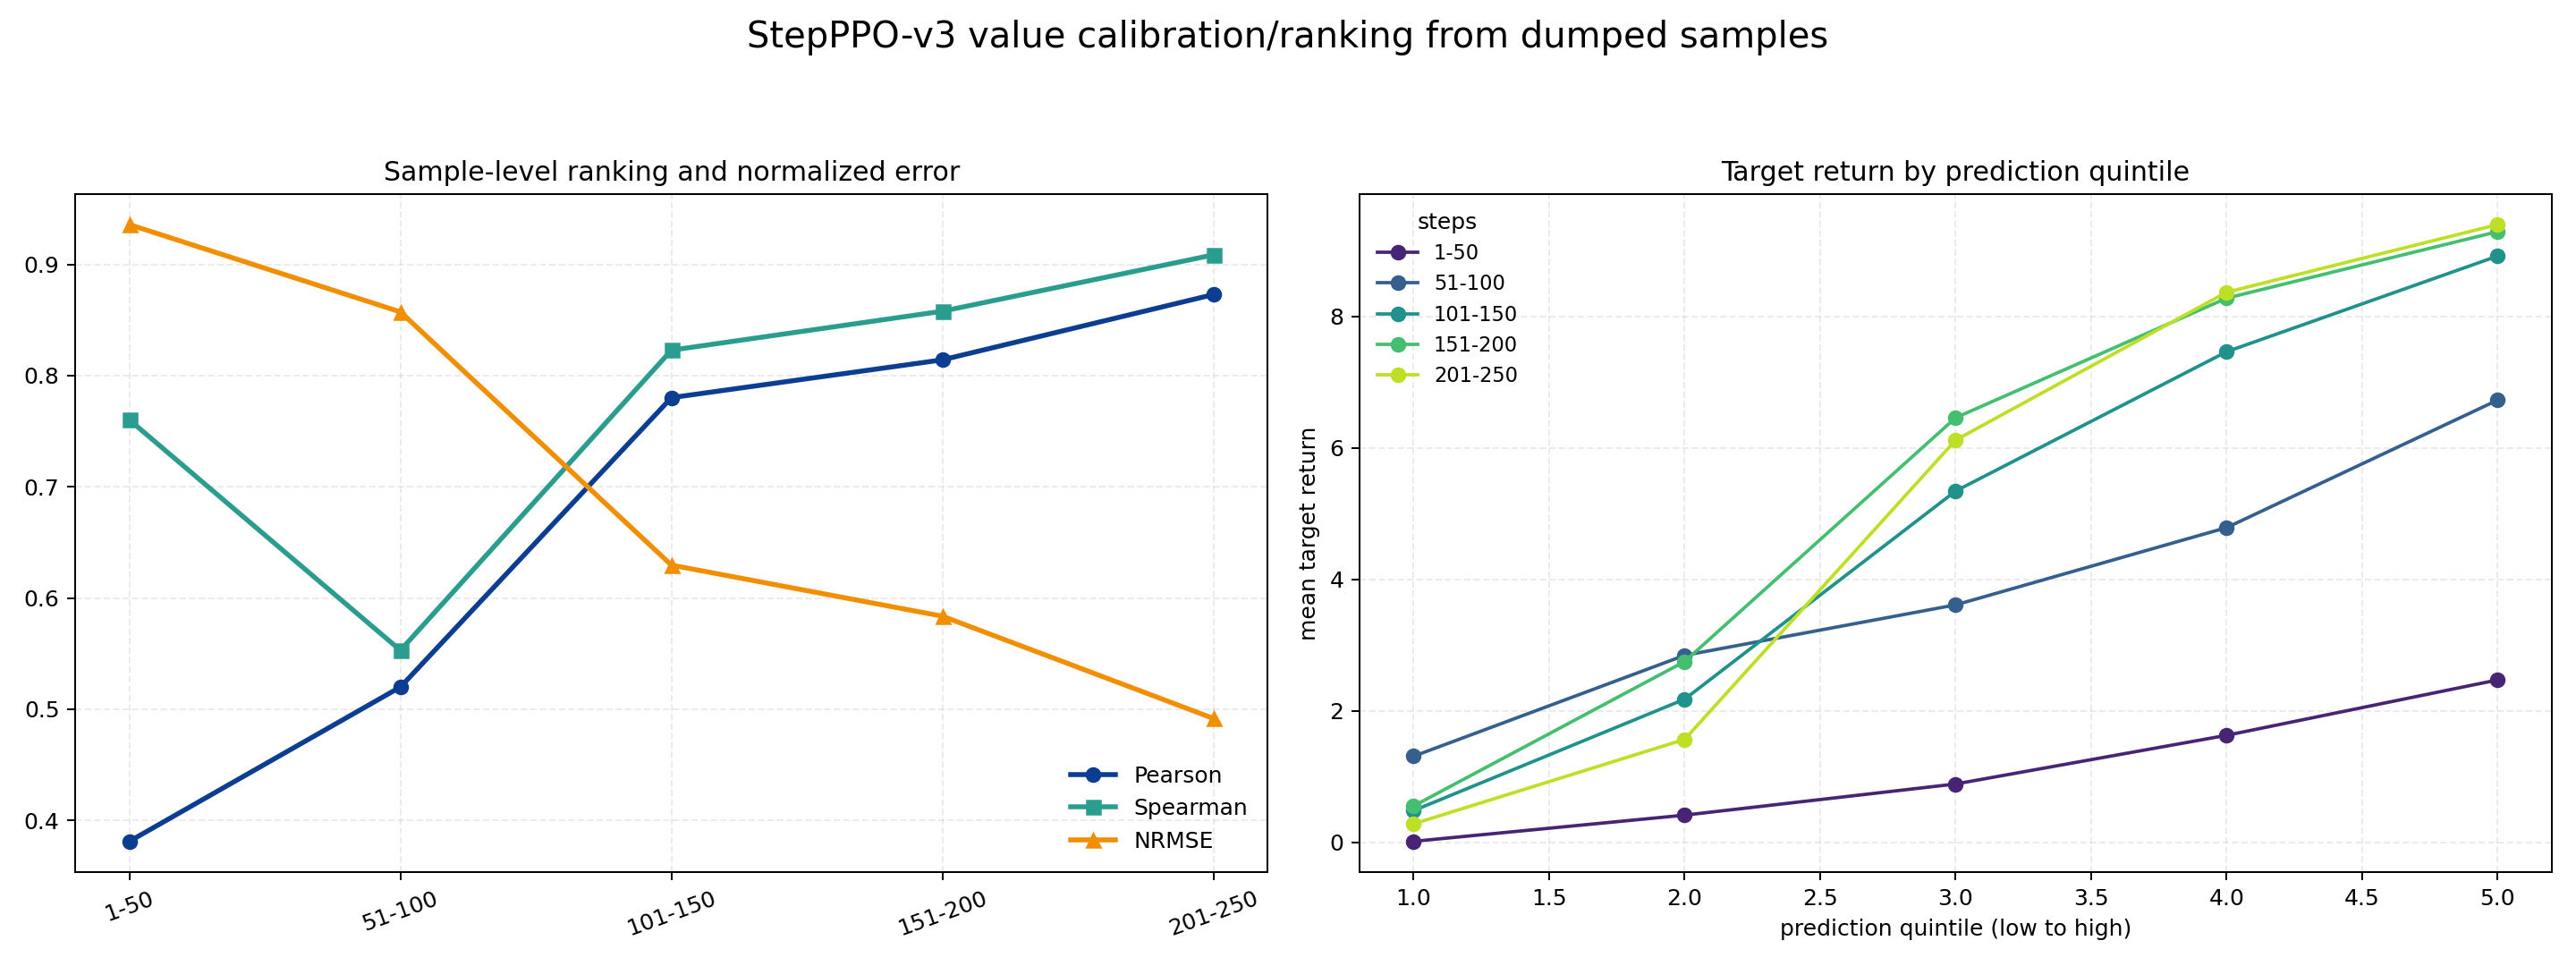
\includegraphics[width=0.92\linewidth]{018_step_ppo_v3_value_calibration_curves.png}
  \caption{基于 dumped sample 的 value ranking/calibration 诊断。}
\end{figure}

\clearpage
\section{对 v3 设计的判断}
这次实验支持如下判断：
\begin{enumerate}
  \item \textbf{selected hidden state 设计是可学习的。}只把 \path{pre_action_last_context_token} 的 hidden state 喂给 value head，并没有阻止 value 学习；后期 ranking、correlation 和 scale matching 都明显改善。
  \item \textbf{step-level GAE return target 有有效信号。}如果 target 主要是噪声，corr 和 Spearman ranking 不应持续上升到 0.8--0.9 区间。
  \item \textbf{detach=false 风险较大。}它让 value loss 直接回传 actor backbone。当前 run 说明这种设置可能诱发 response length drift，从而影响 GiGPO 的行为和成本。
  \item \textbf{当前结果还不支持把 value 直接用于 policy advantage。}value head 已有不错 ranking，但 actor 行为已经受影响；在把 value 接入 advantage 前，需要先稳定 actor 行为。
\end{enumerate}

\section{建议的下一步}
我建议下一轮只围绕“value head 可学习且不影响 GiGPO”继续做最小 ablation：
\begin{itemize}
  \item 跑一个完整 \path{detach_value_backbone=True, value_loss_coef=0.03}，验证是否能保留 value learning，同时消除 response length drift。
  \item 如果 detach=true 学习明显变慢，再试 \path{detach=false} 但降低 \path{value_loss_coef}，例如 0.01 或 0.003。
  \item 把 diagnostics 中的 \path{value_nrmse}、\path{value_corr}、\path{value_std_ratio}、\path{value_full_batch_ev} 写入主日志，而不是只依赖 raw \path{actor/value_loss}。
  \item 把 \path{response_length/clip_ratio} 作为 v3 的 hard safety metric；如果超过 0.1，应优先分析 actor drift，而不是继续解释 value loss。
\end{itemize}

\section{产物位置}
本次新增的分析脚本、曲线和表格如下：
\begin{lstlisting}
EXPS/visualization/plot_step_ppo_v3_complete_analysis.py
EXPS/figures/018_step_ppo_v3_value_learning_curves.png
EXPS/figures/018_step_ppo_v3_policy_vs_gigpo_curves.png
EXPS/figures/018_step_ppo_v3_runtime_resource_curves.png
EXPS/figures/018_step_ppo_v3_value_calibration_curves.png
EXPS/data/018_step_ppo_v3_complete_analysis_summary.txt
EXPS/data/018_step_ppo_v3_policy_window_summary.csv
EXPS/data/018_step_ppo_v3_runtime_window_summary.csv
EXPS/data/018_step_ppo_v3_validation_summary.csv
EXPS/data/018_step_ppo_v3_value_window_summary.csv
EXPS/data/018_step_ppo_v3_value_sample_ranking_summary.csv
EXPS/data/018_step_ppo_v3_value_selected_steps.csv
\end{lstlisting}

\section{最终结论}
v3 的核心问题“value head 能不能稳定学出 step-level value/return target”已经得到比较正面的答案：\textbf{能学，而且后期已经学到很强的 ranking signal 和相当好的 normalized calibration。}

但这次 \path{detach_value_backbone=False} run 暴露出另一个问题：\textbf{value loss 回传 backbone 后，actor 行为并非完全保持 GiGPO baseline，后期 response length drift 很明显。}所以 v3 当前最合理的定位仍然是 auxiliary value-head 验证，而不是更进一步的 policy-advantage 改造。下一步应该优先验证 detach=true 或更小 value loss coefficient，目标是保留 value learning，同时恢复 GiGPO 的 response length、valid action ratio、task score 和 runtime 行为。

\end{document}
